%\documentclass[a4paper]{article}
\usepackage[utf8]{inputenc}
\usepackage[spanish, es-tabla, es-noshorthands]{babel}
\usepackage[table,xcdraw]{xcolor}
\usepackage[a4paper, footnotesep=1.25cm, headheight=1.25cm, top=2.54cm, left=2.54cm, bottom=2.54cm, right=2.54cm]{geometry}
%\geometry{showframe}
%VERIFICAR EL HEAD Y EL FOOT EN
%https://ctan.dcc.uchile.cl/macros/latex/contrib/geometry/geometry.pdf

%\usepackage{lipsum}			%LOREM IPSUM

%\usepackage{wrapfig}		%Wrap figure in text
\usepackage[export]{adjustbox}	%Move images
\usepackage{changepage}			%Move tables

%Font
\usepackage{anyfontsize}	%Font size
% #1 = size, #2 = text
\newcommand{\setparagraphsize}[2]{{\fontsize{#1}{6}\selectfont#2 \par}}		%Cambia el size de todo el parrafo
\newcommand{\setlinesize}[2]{{\fontsize{#1}{6}\selectfont#2}}				%Cambia el font de una oración


%FONTS (IMPORTANTE): Compilar en XeLaTex o LuaLaTeX
\usepackage{fontspec}
%Si sigue sin andar comentar \usepackage[utf8]{inputenc}
%https://ctan.dcc.uchile.cl/macros/unicodetex/latex/fontspec/fontspec.pdf
%https://www.overleaf.com/learn/latex/XeLaTeX

\usepackage{tikz}
\usepackage{amsmath}
\usepackage{amsfonts}
\usepackage{amssymb}
\usepackage{float}
\usepackage{graphicx}
\usepackage{caption}
\usepackage{subcaption}
\usepackage{multicol}
\usepackage{multirow}
\setlength{\doublerulesep}{\arrayrulewidth}
\usepackage{booktabs}

\usepackage{hyperref}
\hypersetup{
    colorlinks=true,
    linkcolor=black,
    filecolor=magenta,      
    urlcolor=blue,
    citecolor=blue,    
}

\newcommand{\captionsection}{\setcounter{figure}{0} \renewcommand{\thetable}{\arabic{section}.\arabic{table}} \renewcommand{\thefigure}{\arabic{section}.\arabic{figure}}}

\newcommand{\captionsubsection}{\setcounter{figure}{0} \renewcommand{\thetable}{\arabic{section}.\arabic{subsection}.\arabic{table}} \renewcommand{\thefigure}{\arabic{section}.\arabic{subsection}.\arabic{figure}}}

\newcommand{\captionsubsubsection}{\setcounter{figure}{0} \renewcommand{\thetable}{\arabic{section}.\arabic{subsection}.\arabic{subsubsection}.\arabic{table}} \renewcommand{\thefigure}{\arabic{section}.\arabic{subsection}.\arabic{subsubsection}.\arabic{figure}}}

%PICTURES AND TABLE INDEX:
\newcommand{\Section}[1]{ \section{#1}\captionsection }
\newcommand{\Subsection}[1]{ \subsection{#1}\captionsubsection }
\newcommand{\Subsubsection}[1]{ \subsubsection{#1}\captionsubsubsection }

%NOTAS GRANDES
\newcommand{\note}[1]{
	\begin{center}
		\huge{ \textcolor{red}{#1} }
	\end{center}
}
%Notas pequeñas
\newcommand{\lnote}[1]{{\fontsize{20}{6}\selectfont\textcolor{green}{#1}}}

\newcommand{\quotes}[1]{``#1''}
\usepackage{array}
\newcolumntype{C}[1]{>{\centering\let\newline\\\arraybackslash\hspace{0pt}}m{#1}}
\usepackage[american]{circuitikz}
\usetikzlibrary{calc}
\usepackage{fancyhdr}
\usepackage{units} 

\graphicspath{{../Prefacio/}{../Acronimos/}{../Introduccion/}{../Objetivos/}{../Definicion/}{../Plan de validacion/}{../Resumen/}}

%COLORES
\definecolor{AzulFoot}{rgb}{0.682,0.809,0.926}	%RGB	%{174,206,235}
\definecolor{AzulInfo}{rgb}{0.180,0.455,0.710}	%RGB	%{46,116,181}
\definecolor{AzulTable}{rgb}{0.302,0.507,0.871}	%RGB	%{68,114,196}
\definecolor{PName}{rgb}{0.353,0.353,0.353}	%RGB	%{90,90,90}

\usepackage{xcolor}
\usepackage{sectsty}
\chapterfont{\color{AzulInfo}}  % sets colour of chapters
\sectionfont{\color{AzulInfo}}  % sets colour of sections
\subsectionfont{\color{AzulInfo}}
\subsubsectionfont{\color{AzulInfo}}

%Header y footer
\usepackage{etoolbox}

\pagestyle{fancy}
\fancyhf{}
\rfoot{\thepage}
\renewcommand{\footrulewidth}{4pt}
\renewcommand{\headrulewidth}{0pt}
\patchcmd{\footrule}{\hrule}{\color{AzulFoot}\hrule}{}{}
%%
%\begin{document}
\Subsection{Validación pruebas funcionales.}
Las siguientes validaciones están relacionadas con el manejo apropiado del tiempo, en particular la siguiente corresponde a \textit{T-INT-FUN-08}
\begin{figure}[H]
\centering
        	\includegraphics[width=\linewidth]{ImagenesValidacion del prototipo/TINTFUN8}
	\caption{Validación de funcionalidad \textit{T-INT-FUN-08}.}
\end{figure}
Se observa que ambos tiempos coinciden por lo que se considera exitosa la prueba.

La siguiente prueba corresponde a \textit{T-INT-FUN-09}. Prueba en la que se desenergiza la \rspi, y luego de esperar el tiempo apropiado se energiza nuevamente y se corrobora que la hora correspondiente al módulo RTC sea correcto.
\begin{figure}[H]
\centering
        	\includegraphics[width=1\linewidth]{ImagenesValidacion del prototipo/TINTFUN9}
	\caption{Validación de funcionalidad \textit{T-INT-FUN-09}.}
\end{figure}
Se observa que el resultado es el esperado.

En esta prueba se valida \textit{T-INT-FUN-11}.
\begin{figure}[H]
\centering
    	\begin{subfigure}{0.49\textwidth}
        	\centering
        	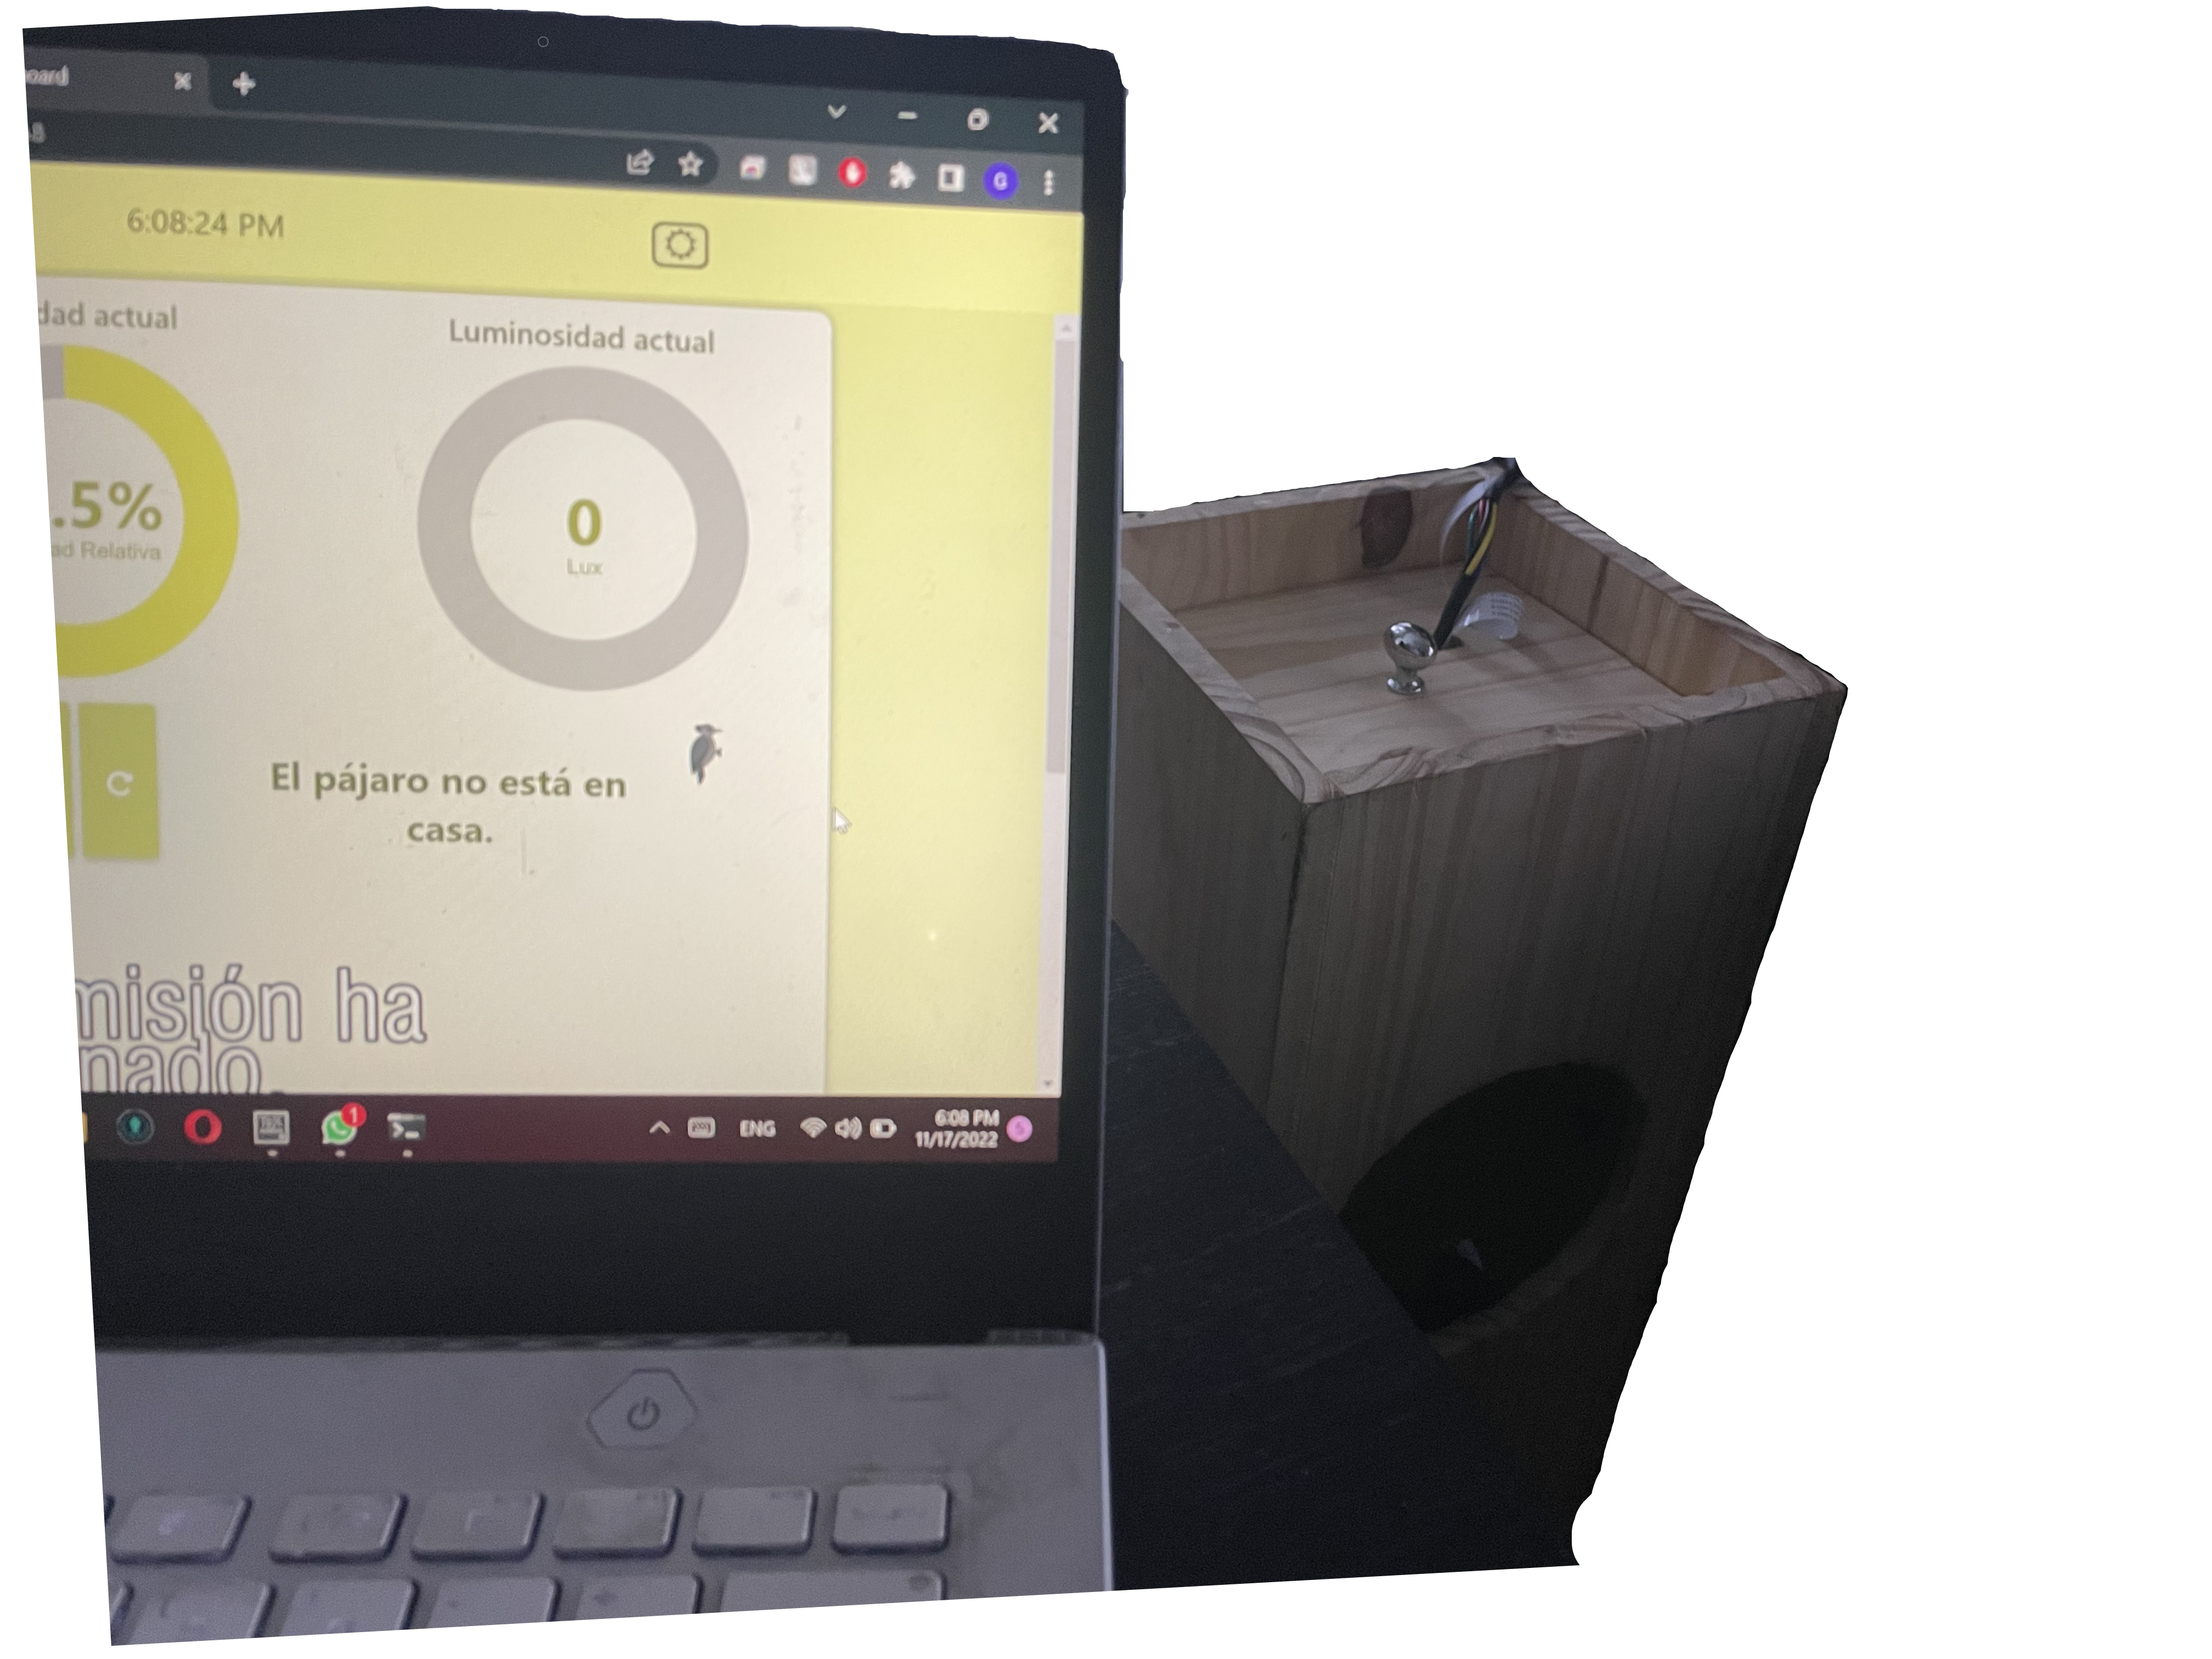
\includegraphics[width=\linewidth]{ImagenesValidacion del prototipo/T-INT-FUN11a}		
			\caption{Beacon fuera del nido.}
        \end{subfigure}\hfill
        \begin{subfigure}{0.49\textwidth}
        	\centering
        	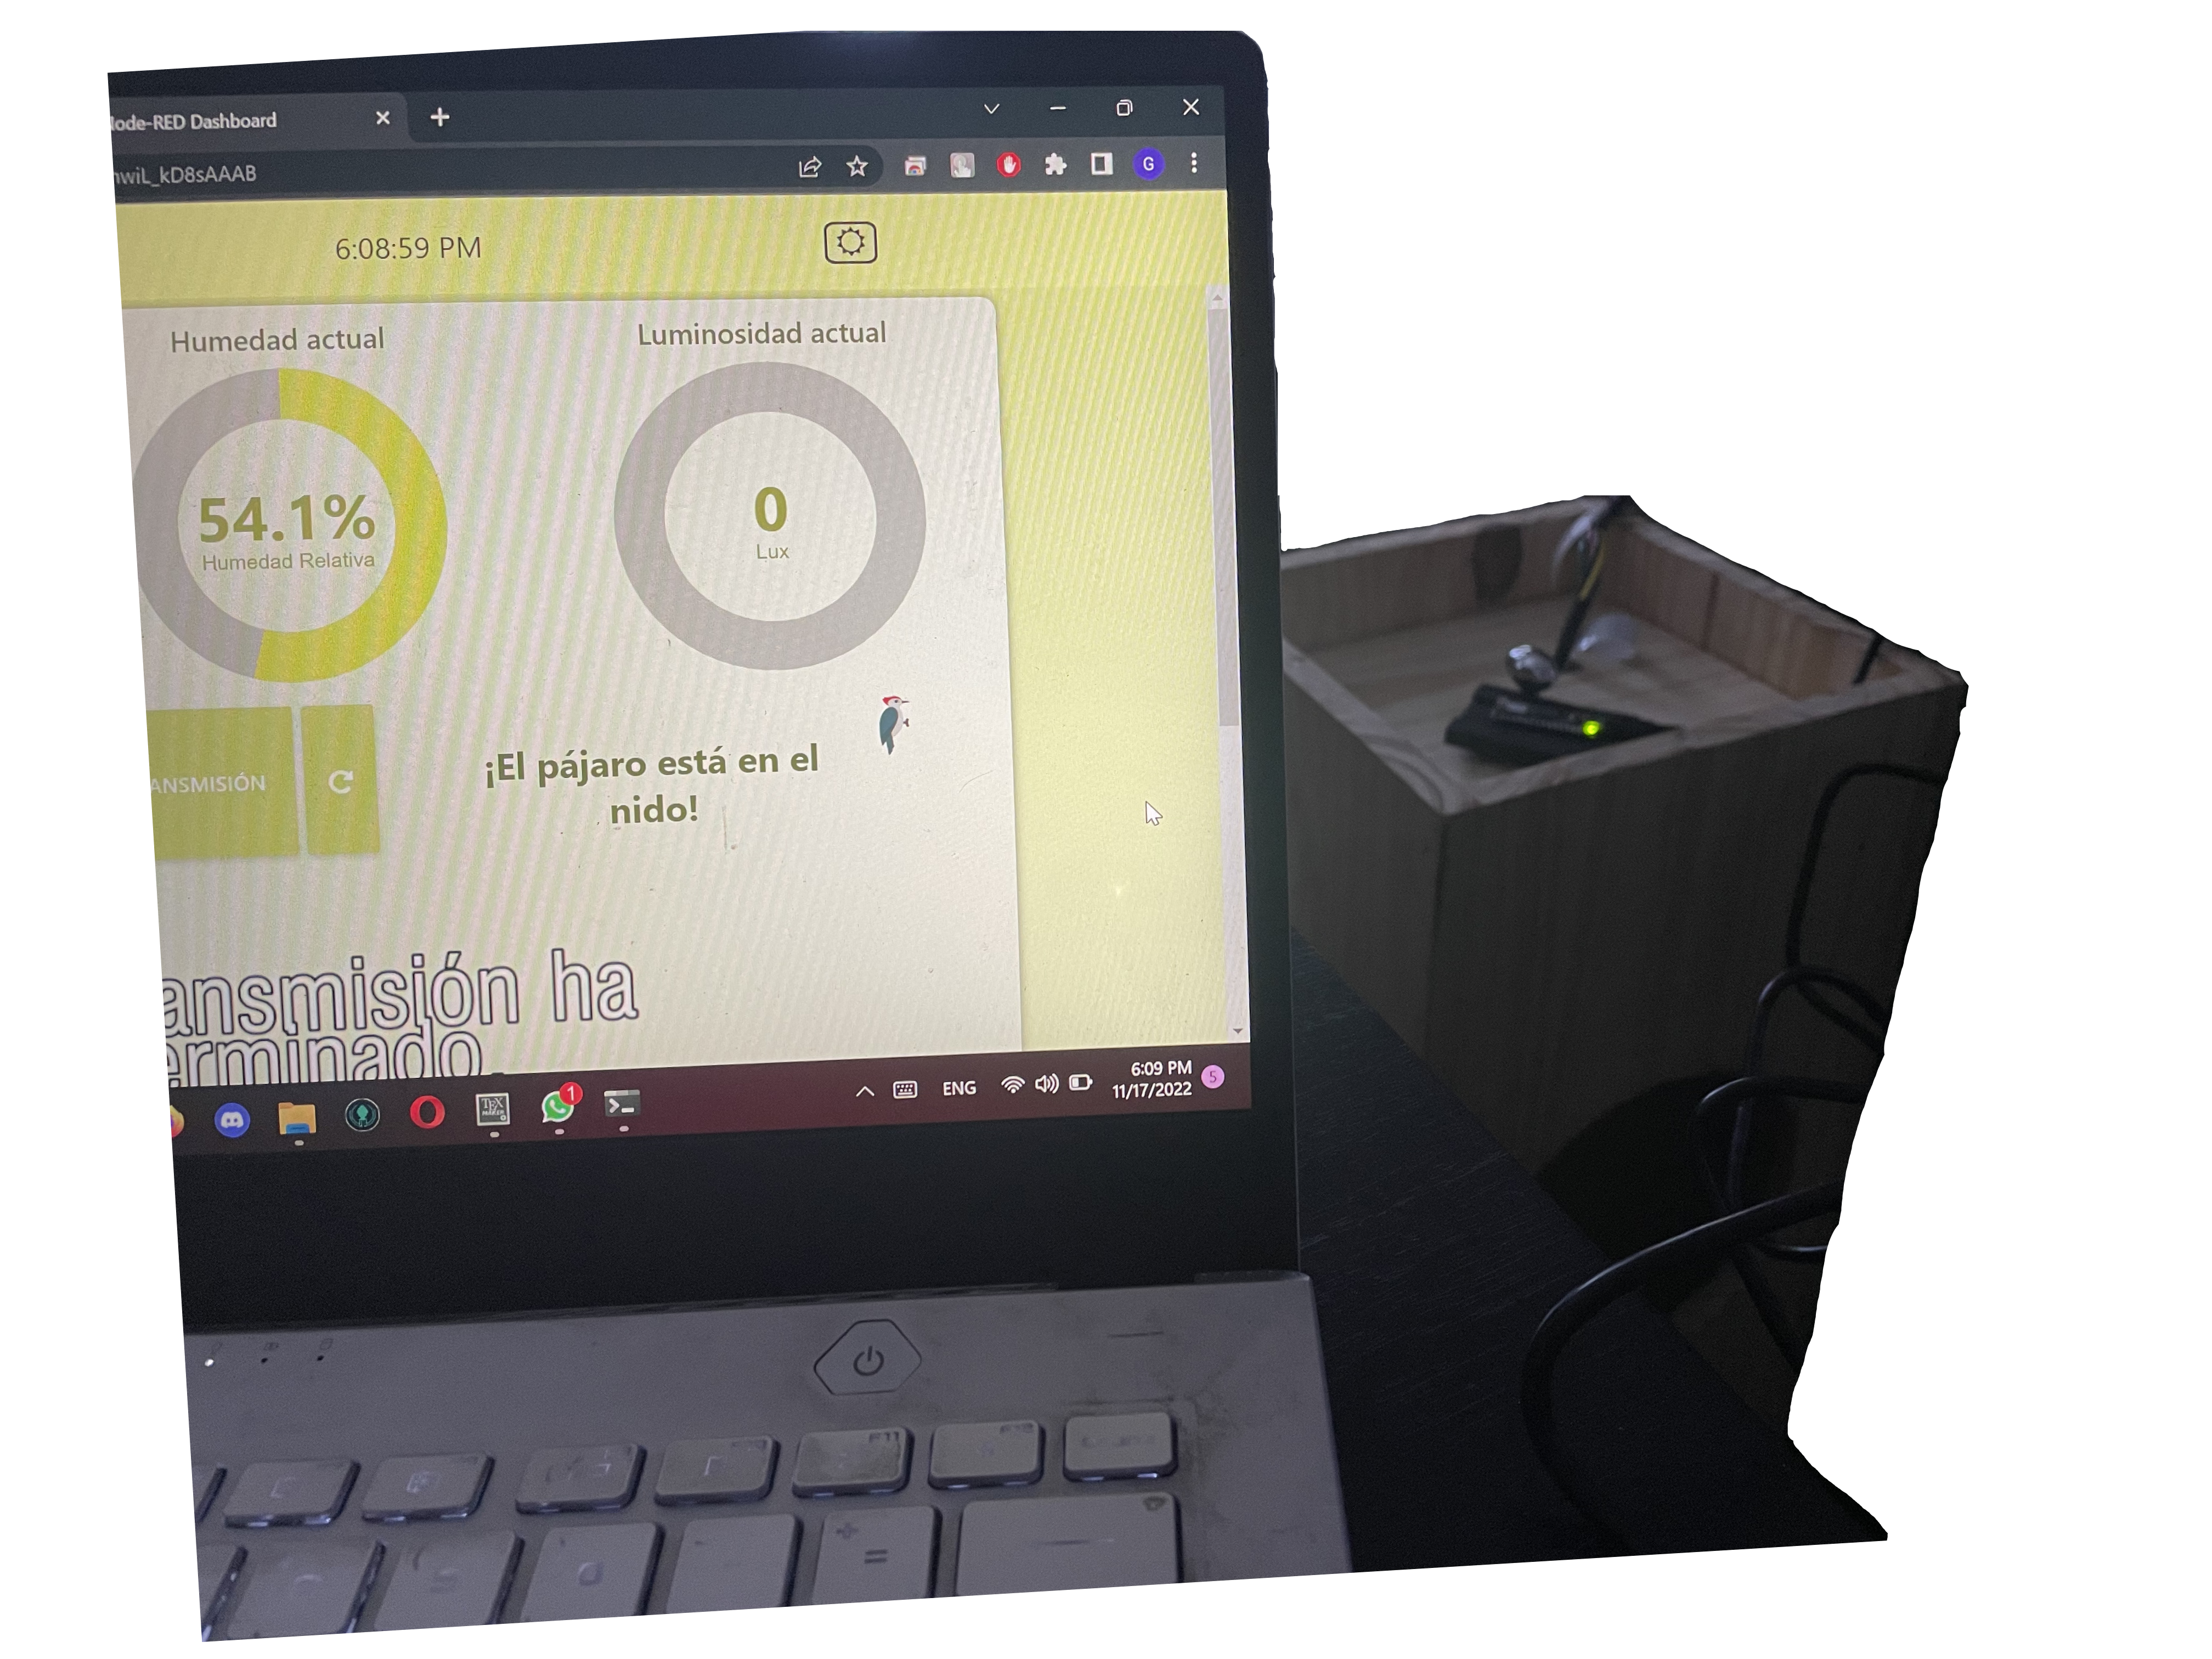
\includegraphics[width=\linewidth]{ImagenesValidacion del prototipo/T-INT-FUN11b}
        	\caption{Beacon en el nido.}
        \end{subfigure}
	\caption{Validación de comunicación \textit{T-INT-FUN-11}.}
\end{figure}

Disponiendo del banco de pruebas \#3, se corroboró mediante observación los tests de funcionalidad \textit{T-INT-FUN-04} y \textit{T-INT-FUN-12}. Se garantizó que la imagen mostrada al usuario sea la adecuada y que se vea de manera fidedigna, es decir que la transmisión sea de calidad y fluida.

\begin{figure}[H]
\centering
    	\begin{subfigure}{0.49\textwidth}
        	\centering
        	\includegraphics[width=\linewidth]{ImagenesValidacion del prototipo/t-int-fun-04-12-1}		
			\caption{Vista de la transmisión en vivo del nido.}
        \end{subfigure}\hfill
        \begin{subfigure}{0.49\textwidth}
        	\centering
        	\includegraphics[width=0.5\linewidth]{ImagenesValidacion del prototipo/t-int-fun-04-12-2}
        	\caption{Imagen del exterior del nido en el momento de la trasmisión.}
        \end{subfigure}
	\caption{Validación de funcionalidad \textit{T-INT-FUN-04} y \textit{T-INT-FUN-12}.}
\end{figure}
\Subsection{Validación Pruebas de Comunicación 1}

\Subsection{Validación Pruebas de Comunicación 2}
En esta sección se realizan las pruebas de comunicación con la computadora de un tercero (Biólogo en campo).
La primer prueba corresponde a \textit{T-INT-COM02-1} la cual corresponde a la capacidad de acceder a  los datos del ave guardados en el nido.
\begin{figure}[H]
\centering
    	\begin{subfigure}{0.49\textwidth}
        	\centering
        	\includegraphics[width=\linewidth]{ImagenesValidacion del prototipo/TINTCOM21a}		
			\caption{Pestaña de descargas.}
        \end{subfigure}\hfill
        \begin{subfigure}{0.49\textwidth}
        	\centering
        	\includegraphics[width=\linewidth]{ImagenesValidacion del prototipo/TINTCOM21b}
        	\caption{Botón de descarga.}
        \end{subfigure}
	\caption{Validación de comunicación \textit{T-INT-COM02-1}.}
\end{figure}

\begin{figure}[H]
\centering
        	\includegraphics[width=1\linewidth]{ImagenesValidacion del prototipo/TINTCOM21}
	\caption{Validación de comunicación \textit{T-INT-COM02-1}.}
\end{figure}
Se observa que los datos descargados que se ven en la izquierda se corresponden con los datos que se encuentran en el nido como se ve a la derecha. Por lo que no hubo una pérdida de datos.
Adicionalmente se utilizó una función de \textit{hash} para comparar los contenidos de ambos archivos y fehacientemente comprobar que son el mismo archivo. 

Se procede a realizar la validación correspondiente a \textit{T-INT-COM02-3}. En esta prueba se de verificar la existencia del archivo \textit{BirdData} luego descargarlo y al acceder nuevamente a la \rspi comprobar que el archivo \textit{BirdData} fue borrado exitosamente.
\begin{figure}[H]
\centering
        	\includegraphics[width=1\linewidth]{ImagenesValidacion del prototipo/TINTCOM23}
	\caption{Validación de comunicación \textit{T-INT-COM02-3}.}
\end{figure}



\Subsection{Validación pruebas de seguridad}
Se dispuso del banco de pruebas \#1 para analizar la aplicabilidad de \textit{T-RAM-SEG-01}. El acceso tanto a la interfaz gráfica del usuario como la del administrador se encuentran restringidas para cualquiera que no posea las credenciales adecuadas.

\begin{figure}[H]
\centering
    	\begin{subfigure}{0.49\textwidth}
        	\centering
        	\includegraphics[width=\linewidth]{ImagenesValidacion del prototipo/t-ram-seg-01-1}		
			\caption{Autenticación de usuario para la interfaz gráfica.}
        \end{subfigure}\hfill
        \begin{subfigure}{0.49\textwidth}
        	\centering
        	\includegraphics[width=\linewidth]{ImagenesValidacion del prototipo/t-ram-seg-01-2}
        	\caption{Autenticación de administrador para la interfaz gráfica.}
        \end{subfigure}
	\caption{Validación de seguridad \textit{T-RAM-SEG-01}.}
\end{figure}

Se obtuvo un resultado mejor del esperado ya que el hecho de emplear una red \wifi para conectar la unidad del nido con el usuario también requiere del uso de una contraseña. Esto agrega una capa de seguridad extra al sistema.


%\end{document}



